%----------------------------------------------------------------------------------------
%	PACKAGES AND THEMES
%----------------------------------------------------------------------------------------

\documentclass[aspectratio=169]{beamer}

\setbeamertemplate{caption}[numbered]
\usepackage{times}

%\usepackage{textpos}
\mode<presentation> {
	
	% The Beamer class comes with a number of default slide themes
	% which change the colors and layouts of slides. Below this is a list
	% of all the themes, uncomment each in turn to see what they look like.
	
	%\usetheme{default}
	%\usetheme{AnnArbor}
	%\usetheme{Antibes}
	%\usetheme{Bergen}
	%\usetheme{Berkeley}
	%\usetheme{Berlin}
	\usetheme{Boadilla}
	%\usetheme{CambridgeUS}
	%\usetheme{Copenhagen}
	%\usetheme{Darmstadt}
	%\usetheme{Dresden}
	%\usetheme{Frankfurt}
	%\usetheme{Goettingen}
	%\usetheme{Hannover}
	%\usetheme{Ilmenau}
	%\usetheme{JuanLesPins}
	%\usetheme{Luebeck}
	%\usetheme{Madrid}
	%\usetheme{Malmoe}
	%\usetheme{Marburg}
	%\usetheme{Montpellier}
	%\usetheme{PaloAlto}
	%\usetheme{Pittsburgh}
	%\usetheme{Rochester}
	%\usetheme{Singapore}
	%\usetheme{Szeged}
	%\usetheme{Warsaw}
	
	% As well as themes, the Beamer class has a number of color themes
	% for any slide theme. Uncomment each of these in turn to see how it
	% changes the colors of your current slide theme.
	
	%\usecolortheme{albatross}
	%\usecolortheme{beaver}
	%\usecolortheme{beetle}
	%\usecolortheme{crane}
	\usecolortheme{dolphin}
	%\usecolortheme{dove}
	%\usecolortheme{fly}
	%\usecolortheme{lily}
	%\usecolortheme{orchid}
	%\usecolortheme{rose}
	%\usecolortheme{seagull}
	%\usecolortheme{seahorse}
	%\usecolortheme{whale}
	%\usecolortheme{wolverine}
	\usefonttheme{serif}
	\usepackage[utf8]{inputenc}
	\usepackage{mathptmx}
	\usepackage{amsmath}
	\usepackage{amsfonts}
	\usepackage{amssymb}
	\usepackage{color}
	\usepackage{url}
        \usepackage{wrapfig}
	\usepackage{multirow}
	\usepackage{multicol}
	\usepackage{booktabs}
	\usepackage{graphicx}
	\usepackage{array}
	\usepackage{arydshln}
	\usepackage{mathtools}
	\usepackage{chngpage}
	\usepackage{url}
	\usepackage{setspace}
	\usepackage{bigstrut}
	\usepackage{tabularx}
	\usepackage{bm}
	\usepackage{bigstrut}
        \usepackage{epsfig}
        \usepackage{epstopdf}
        \usepackage{hyperref}
        \usepackage{amsfonts,amsmath,bbm,bm,xcolor,booktabs,hyperref,amsthm}
	%\setbeamertemplate{footline} % To remove the footer line in all slides uncomment this line
	%\setbeamertemplate{footline}[pagenumber] % To replace the footer line in all slides with a simple slide count uncomment this line
	
	\setbeamertemplate{navigation symbols}{} % To remove the navigation symbols from the bottom of all slides uncomment this line
}
\usepackage{bigstrut}
\usepackage{caption}
\usepackage{subfig}
\usepackage{float}
\usepackage{graphicx} % Allows including images
\usepackage{graphics}
\usepackage{epsfig}
\usepackage{epstopdf}
\usepackage{booktabs} % Allows the use of \toprule, \midrule and \bottomrule in tables
\usepackage{natbib}
\usepackage{setspace}
\usepackage{comment}
\usepackage{multirow}
\usepackage{multicol}
\usepackage{bigstrut}
\usepackage{lscape,tikz-qtree}
\usetikzlibrary{arrows,shapes,positioning,shadows,trees}

\graphicspath{{figures/}} 

\newcounter{researchquestion}
\setcounter{researchquestion}{0}

% Define the environment for the research questions
\newenvironment{researchquestion}{%
    \refstepcounter{researchquestion}%
    \par\medskip\noindent%
    \textbf{RQ\theresearchquestion.}~%
}{\medskip}

\linespread{1}
\newenvironment{myenv}[1]
{\begin{spacing}{#1}}
	{\end{spacing}}

\AtBeginSection[]
{
	%\ifthenelse{\boolean{sectiontoc}}{
	%    \begin{frame}<beamer>{Gliederung}
	%      \tableofcontents[currentsection]
	%    \end{frame}
	%  }
	%\newcommand{\toclesssection}[1]{
	%  \setboolean{sectiontoc}{false}
	%  \section{#1}
	%  \setboolean{sectiontoc}{true}
	%}
	
	%\begin{frame}[noframenumbering]  
	%	\frametitle{Outline} \tableofcontents[currentsection, subsectionstyle=hide] 
	%\end{frame}
	
	%\addtocounter{framenumber}{-1}
}

\AtBeginSection[]
{\begin{frame}  

  \frametitle{Outline} \tableofcontents[currentsection, subsectionstyle=hide] 

\end{frame}
\addtocounter{framenumber}{-1}
}

%----------------------------------------------------------------------------------------
%	TITLE PAGE
%----------------------------------------------------------------------------------------
	
	%\begin{frame}
	%\frametitle{Overview} % Table of contents slide, comment this block out to remove it
	%\tableofcontents % Throughout your presentation, if you choose to use \section{} and \subsection{} commands, these will automatically be printed on this slide as an overview of your presentation
	%\end{frame}
	
	%----------------------------------------------------------------------------------------
	%	PRESENTATION SLIDES
	%----------------------------------------------------------------------------------------
	
	%------------------------------------------------

\title[Constructing hierarchical time series through clustering]{Constructing hierarchical time series through clustering: \\Is there an optimal way for forecasting?}
%\vspace{8mm}
%\author{{\bf Han Li$^*$ and Colin O'Hare$^{\dagger}$} \vspace{6mm}\\\vspace{0.05cm} \small $^*$ARC Centre of Excellence in Population Ageing Research (CEPAR), UNSW \vspace{2mm}\\ \small $^\dagger$Department of Econometrics and Business Statistics, Monash University}
	
\vspace{-8in}	
	
\author[Bohan Zhang]{Bohan Zhang$^{1}$, Anastasios Panagiotelis$^{2}$, and Han Li$^{3}$} % Your name
	\institute[] % Your institution as it will appear on the bottom of every slide, may be shorthand to save space
	%{\small {$^1$ \small  Department of Statistics and Department of Mathematics\\ \textbf{Purdue University}}\\ 
	 %\vskip 0.2cm	
  	{\small {$^1$ \small School of Economics and Management, Beihang University}
   \vskip 0.2cm
	\small {$^2$ Discipline of Business Analytics, Business School, University of Sydney}	
    \vskip 0.2cm
  	\small {$^3$ \small Centre for Actuarial Studies, Department of Economics, University of Melbourne}
   \vskip 0.5cm
\textbf{The 44th International Symposium on Forecasting, Dijon, France}
}
	\date{30 June - 3 July, 2024} % Date, can be changed to a custom date

	%\logo{\includegraphics[height=0.7cm]{Figures/logo_all.png}\vspace{-0.3cm}}
 
%	\logo{\includegraphics[height=3.5cm]{Doc1}\vspace{-2cm}}
	
	
\begin{document}
	
\begin{frame}
\titlepage
% \vspace{0.3cm}

\end{frame}
				


 
% \begin{frame}{Outline of the presentation}
% 	\large
% 	\begin{enumerate}
% 		\item \color {blue} What are we trying to measure, and why?
% 		\vspace{0.08in}
%             \item Data description
%             \vspace{0.08in}
% 		\item \color {blue} What modelling procedures are used?
%   		\begin{itemize}
% 		\vspace{0.02in}
% 			\item Standardisation and smoothing
% 		\vspace{0.02in}
% 			\item Linear regression and time series modelling
% 		\vspace{0.02in}
% 			\item Forecast reconciliation
% 		\end{itemize}
% 		\vspace{0.02in}
% 		\item \color {blue} What do the results look like?\vspace{0.08in}		
% 		\item \color {blue} Questions and discussions
 
% 		%\vspace{0.08in}
% 		%\item  \color {blue} 
				
% 	\end{enumerate}
% \end{frame}

%------------------------------------------------

\begin{frame}{Outline of the presentation}

\tableofcontents 
\end{frame}

\section{Hierarchical forecasting and forecast reconciliation}

\begin{frame}{Hierarchical forecasting and forecast reconciliation}
\begin{figure}
    \centering
    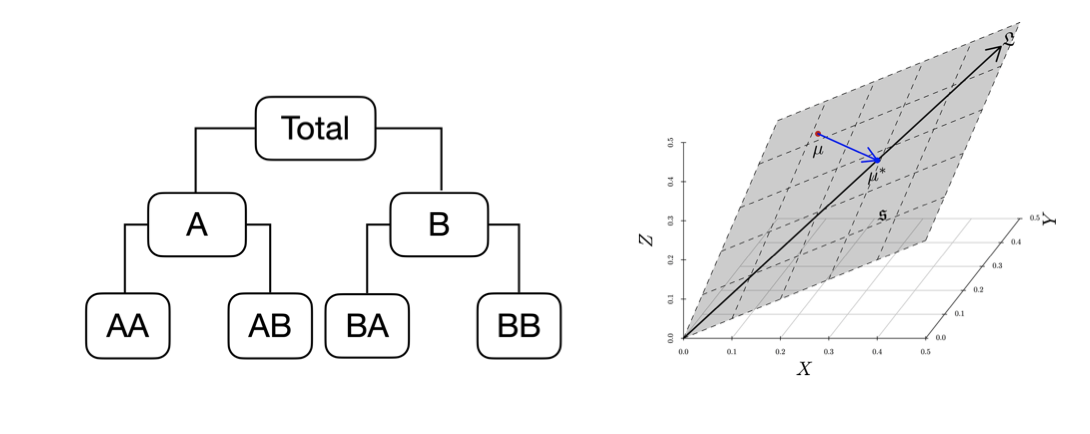
\includegraphics[width=0.7\textwidth]{hts.png}    
\end{figure}
\vspace{-0.7cm}
\begin{itemize}
    \item (Cross-sectional) Hierarchical time series is multivariate time series whose observations at time $t$ respect \textbf{aggregation constraints}.
    \item Hierarchical forecasting produces \textit{coherent} forecasts for hierarchical time series.
    \item Forecast reconciliation projects incoherent base forecasts of all time series onto the coherent subspace (\citealp{panagiotelisForecastReconciliationGeometric2021}).
\end{itemize}

\end{frame}

\begin{frame}{Forecast reconciliation: the forecast combination perspective}

	\begin{itemize}
		\item Forecast reconciliation can be interpreted from the forecast combination perspective (\citealp{hollymanUnderstandingForecastReconciliation2021,difonzoForecastCombinationbasedForecast2024}).
		\item Reconciled forecasts are weighted combination of ``direct'' and ``indirect'' base forecasts. 
		\[
			\tilde{y}_{AA} = w_1 \hat y_{AA} + w_2 (\hat y_{A} -\hat y_{AB}) + w_3 (\hat y_{Total} - \hat y_{AB} - \hat y_{BA} - \hat y_{BB})
		\]
	
		\item Could we employ {\color{red} more ``indirect'' forecasts} and improve forecast accuracy?
		\begin{itemize}
			\item Add middle-level series.
		\end{itemize}
		\item Could we find {\color{red} more accurate ``indirect'' forecasts} and improve forecast accuracy?
		\begin{itemize}
			\item Cluster similar time series (\citealp{liForecastReconciliationApproach2019,pangHierarchicalElectricityTime2022,matteraImprovingOutofSampleForecasts2023}).
			\item The rationale behind clustering lies in grouping time series with similar patterns together, thereby creating middle-level series with enhanced signals and consequently, improved forecastability.
		\end{itemize}
	\end{itemize}
		
	\end{frame}
	

%------------------------------------------------
\section{Research questions}
%------------------------------------------------


\begin{frame}{Research questions}
	\begin{researchquestion}
		In terms of forecast performance, can {\color{red} the use of middle level series lead to improvement} compared to a two-level hierarchy (consisting of only top and bottom time series)? If so, is it possible to {\color{red} construct hierarchies in a data-driven way} that leads to further improvements in forecast accuracy?
	\end{researchquestion}

	\begin{figure}
		\centering
		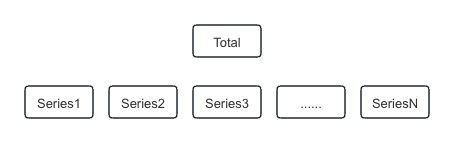
\includegraphics[width=0.45\textwidth]{RQ1-l.png}
		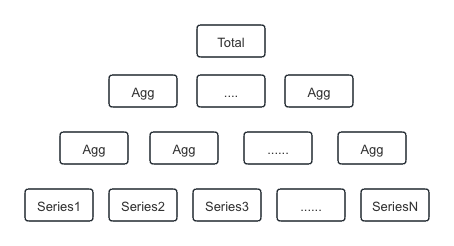
\includegraphics[width=0.45\textwidth]{RQ1-r.png}
	\end{figure}

	\begin{itemize}
		\item Does creating ``Agg''s improve forecast accuracy?
		\item How to construct ``Agg''s in a data-driven approach?
	\end{itemize}

\end{frame}


\begin{frame}{Research questions}

	The increased accuracy when using data-driven approach may be attributed to two factors.

	\begin{itemize}
		\item {\color{red} Grouping}: some correct subsets of series are chosen to form new middle-level series.
		\item {\color{red} Structure}: the number of middle-level series, the depth of the hierarchy, and the distribution of group sizes in the middle layer(s).
	\end{itemize}


	\begin{researchquestion}
		Should the improved accuracy of clustering-based methods be attributed to grouping together similar time series, or to the structure of the hierarchy?
	\end{researchquestion}
\end{frame}


\begin{frame}{Research questions}
	
	With {\color{red} multiple hierarchies available} and inspired by the forecast combination literature (\citealp{wangForecastCombinations50year2022}), we consider the last research question:

	\begin{researchquestion}
		Does an equally-weighted combination of reconciled forecasts derived from multiple hierarchies improve forecast reconciliation performance?
	\end{researchquestion}
\end{frame}



\section{Time series clustering-based forecast reconciliation}

\begin{frame}{Time series clustering-based forecast reconciliation}
	To the best of our knowledge, four studies have attempted to improve forecast accuracy in a reconciliation setting by constructing middle levels of the hierarchy using time series clustering.

	\begin{itemize}
		\item \cite{pangHierarchicalElectricityTime2018} and \cite{pangHierarchicalElectricityTime2022} propose to employ K-means algorithm to group similar electricity and solar power time series.
		\item \cite{liForecastReconciliationApproach2019} apply agglomerative hierarchical clustering to cause-of-death time series.
		\item \cite{matteraImprovingOutofSampleForecasts2023} utilize Partition Around Medoids algorithms to unveil underlying structures in stock price indexes.
	\end{itemize}

	We consider various approaches based on three key components, namely {\color{red} time series representations}, {\color{red} distance measures}, and {\color{red} clustering algorithms}.
\end{frame}

\begin{frame}{Time series representations}

	The time series representation refers to the object that acts as an input for time series clustering. We consider four representations:
	\begin{itemize}
		\item {\color{red} Raw time series}.
		\item {\color{red} In-sample one-step-ahead forecast error}. A key step in MinT reconciliation is to estimate $\boldsymbol{W}_h$ based on in-sample forecast error.
		\item {\color{red} Time series features of raw time series}.
		\item {\color{red} Time series features of in-sample one-step-ahead forecast error}. 
		\begin{itemize}
			\item Features are low dimensional representation of time series, and have been used in various tasks such as clustering and forecasting.
			\item $56$ features calculated by the \texttt{tsfeatures} package in R are included.
		\end{itemize}
	\end{itemize}
\end{frame}


\begin{frame}{Distance measures}

	All clustering algorithms we consider require a distance to be defined between the objects that act as inputs to the algorithm. 
	
	We consider two widely applied distance measures: {\color{red} Euclidean distance} (combined with PCA to reduce dimensionality) and {\color{red} dynamic time warping (DTW)}.
	
	
\end{frame}

\begin{frame}{Clustering algorithms}
	We focus on two clustering algorithms:

	\begin{itemize}
		\item {\color{red} Partitioning around medoids}, which is an algorithm to find a local minimum for the $k$-medoids problem.
		\item {\color{red} Agglomerative hierarchical clustering} with Ward's linkage.
	\end{itemize}

	\begin{figure}
		\centering
		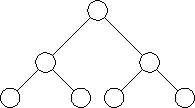
\includegraphics[width=0.35\textwidth]{pamcluster.pdf}
		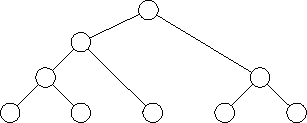
\includegraphics[width=0.35\textwidth]{aggcluster.pdf}
	\end{figure}

	\begin{itemize}
		\item PAM (left) constructs {\color{red} a simple hierarchy with a single middle level}, while hierarchical clustering (right) generates {\color{red} multiple nested middle levels}.
		\item As the number of bottom-level series increases, these differences become increasingly pronounced, with potential implications for forecast reconciliation.
	\end{itemize}
\end{frame}

\begin{frame}{Summary}
	\begin{table}[h!]
		\caption{\label{tab:P3_methods} Details of the 12 clustering approaches considered.}
		\centering
		\resizebox{\textwidth}{!}{
		\begin{tabular}{rcrrr}
			\toprule
			Approach & Dimension reduction & Representation & Distance measure & Clustering algorithm  \\ \midrule
			TS-EUC-ME &  Yes & Time series  & Euclidean & $k$-medoids \\
			ER-EUC-ME & Yes& In-sample  error  & Euclidean & $k$-medoids \\
			TSF-EUC-ME & Yes& Time series features  & Euclidean & $k$-medoids \\
			ERF-EUC-ME & Yes& In-sample error features  & Euclidean & $k$-medoids \\
			TS-EUC-HC & Yes& Time series  & Euclidean & Hierarchical   \\ 
			ER-EUC-HC & Yes& In-sample error  & Euclidean & Hierarchical   \\ 
			TSF-EUC-HC & Yes& Time series features  & Euclidean & Hierarchical   \\ 
			ERF-EUC-HC & Yes& In-sample error features  & Euclidean & Hierarchical  \\
			TS-DTW-ME & No& Time series  & DTW & $k$-medoids \\
			TS-DTW-HC & No& In-sample error  & DTW & Hierarchical  \\
			ER-DTW-ME & No& Time series  & DTW & $k$-medoids \\
			ER-DTW-HC & No& In-sample error  & DTW & Hierarchical 
			 \\\bottomrule
		\end{tabular}}
		\end{table}
\end{frame}

\section{Data description}

\begin{frame}{Australian tourism dataset}
	\begin{figure}
		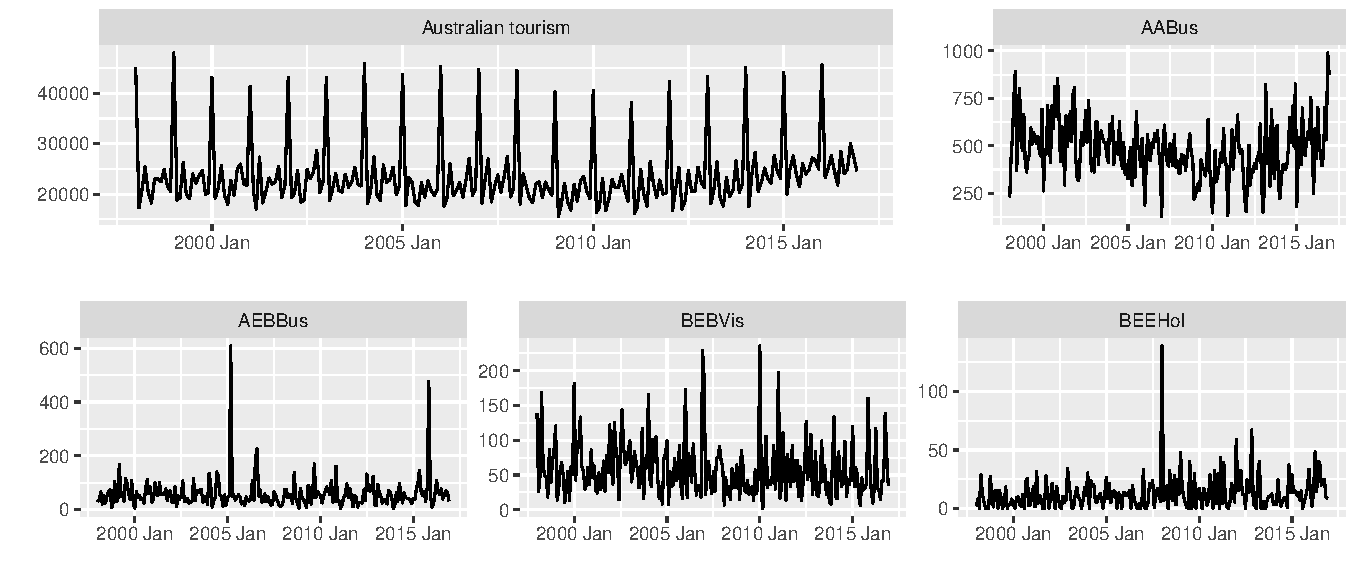
\includegraphics[width=0.8\textwidth]{../manuscript/figures/tourism.pdf}
	\end{figure}
	\begin{itemize}
		\item Monthly Australian domestic tourism dataset, covering the period from January 1998 to December 2016 (\citealp{wickramasuriyaOptimalForecastReconciliation2019}).
		\item Consists of $555$ time series with $304$ of those at the bottom level. The middle-level series are constructed based on state, region, city and travel purpose.
	\end{itemize}
	
\end{frame}

\begin{frame}{U.S. cause-of-death count dataset}
	\begin{figure}
		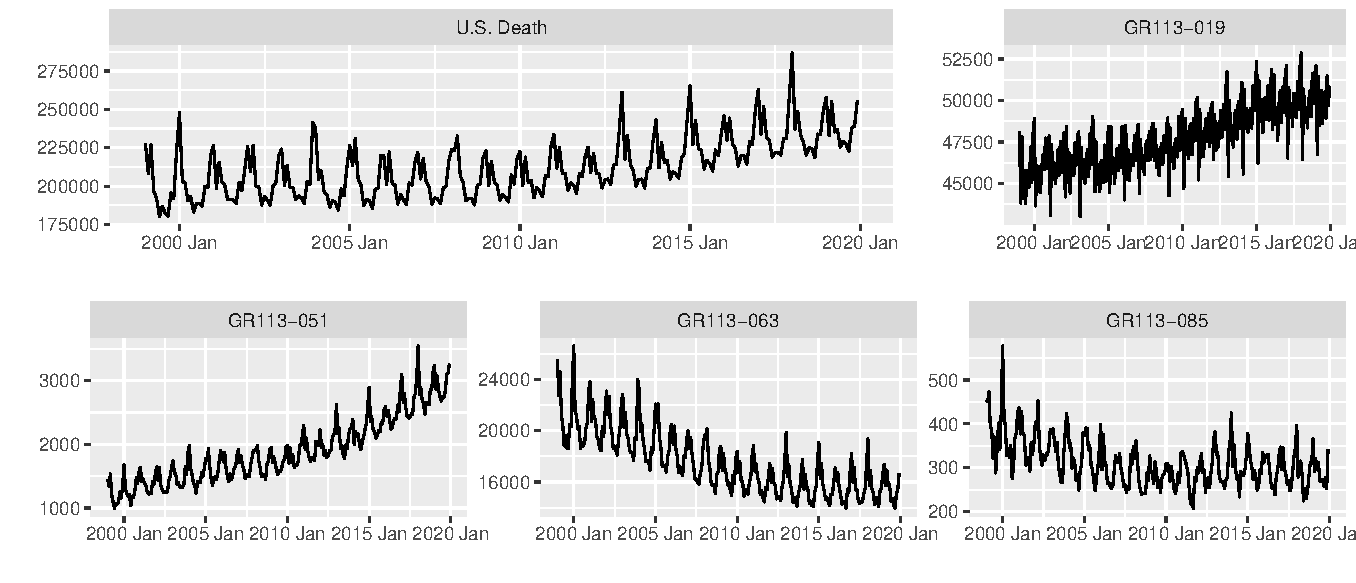
\includegraphics[width=0.8\textwidth]{../manuscript/figures/mortality.pdf}
	\end{figure}
	\begin{itemize}
		\item Monthly cause-specific death count data of U.S. for the period between January 1999 and December 2019.
		\item Consists of $120$ time series, with $98$ of those being bottom-level series. The middle-level series are constructed based on major cause-of-death groups.
	\end{itemize}
\end{frame}

\section{Improving forecast performance via hierarchy augmentation}

\begin{frame}{Evaluation}

	\begin{itemize}
		\item We employ the expanding window strategy, resulting in $121$ $12$-step-ahead forecasts for tourism dataset, and $145$ $12$-step-ahead forecasts for mortality dataset.
		\item We only focus on the total series and bottom-level series.
		\item Forecast accuracy is evaluated based on average RMSSE of all time series (total and bottom).
		\item {\color{red} Three benchmarks}: Base forecast, Two-level hierarchy (total and bottom), Natural hierarchy (constructed based on attributes of the bottom-level series)
	\end{itemize}
	
\end{frame}

\begin{frame}{Cluster hierarchies vs benchmarks}
	
	\begin{figure}
		\centering
		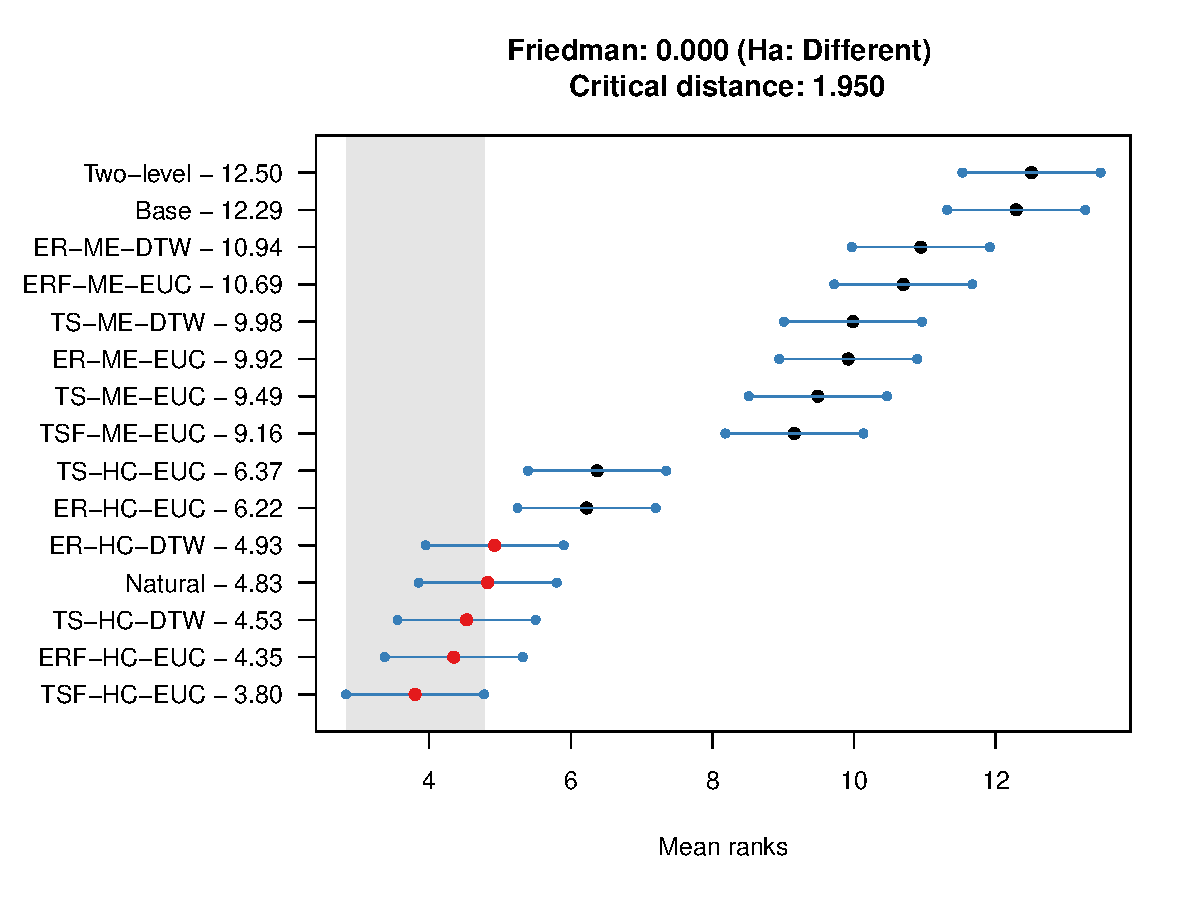
\includegraphics[width=0.4\textwidth]{../manuscript/figures/hierarchy_rmsse/tourism/P3_mcb_benchmarks_h12.pdf}
		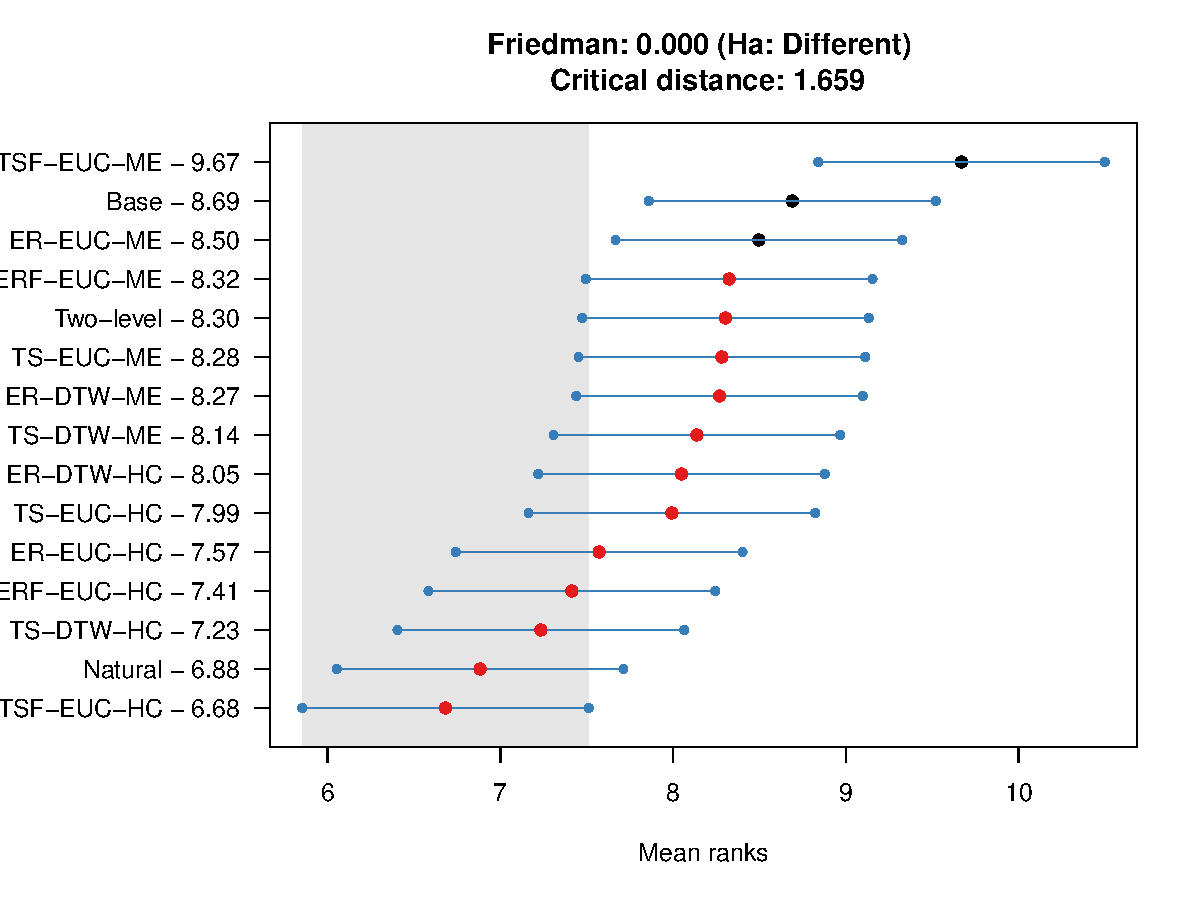
\includegraphics[width=0.4\textwidth]{../manuscript/figures/hierarchy_rmsse/mortality/P3_mcb_benchmarks_h12.pdf}
		\caption{Average ranks and 95\% confidence intervals for twelve cluster hierarchies and three benchmarks on tourism dataset (left) and mortality dataset (right) based on MCB test.}
	\end{figure}

\end{frame}

\begin{frame}{Cluster hierarchies vs benchmarks}

	\begin{itemize}
		\item The {\color{red} natural hierarchies} provide better results than the base forecasts and the two-level hierarchies, and {\color{red} comparable results with cluster hierarchies}.
		\item For tourism dataset, {\color{red} ten out of twelve} cluster hierarchies significantly outperform two-level hierarchy. However for mortality dataset, none of the cluster hierarchies significantly outperform two-level hierarchy.
		\begin{itemize}
			\item The performance of clustering-based forecast reconciliation depend on the characteristics of bottom-level series.
			\item The tourism dataset predominately contains {\color{red} volatile and noisy} bottom-level time series with weak trend and seasonality. 
			\item The bottom-level series in mortality dataset exhibit {\color{red} stronger trend and seasonality patterns}, meaning that the addition of middle-level series is less beneficial.
		\end{itemize}
		\item The hierarchies constructed via {\color{red} hierarchical clustering} algorithms outperform the hierarchies based on {\color{red} k-medoids }when using the same representation and distance metric.
	\end{itemize}
\end{frame}

\begin{frame}{Disentangling grouping and structure}
	To assess whether ``grouping'' or ``structure'' has relatively more importance, we propose to construct {\color{red}``twin'' hierarchies} constructed by {\color{red}randomly permuting the bottom-level series}.

	\begin{figure}
		\centering
		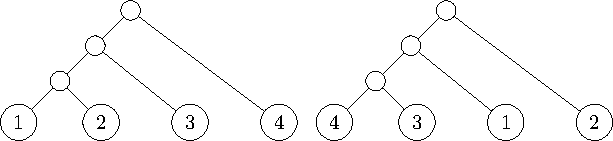
\includegraphics[width=0.8\textwidth]{../manuscript/figures/aggcluster_random.pdf}
		\caption{Examples of a given hierarchy and its “twin”.}
	\end{figure}
\end{frame}

\begin{frame}{Natural hierarchy vs its twins}

We construct $100$ twin hierarchies for each of the two natural hierarchies and compare their performance.

\begin{figure}
	\centering
	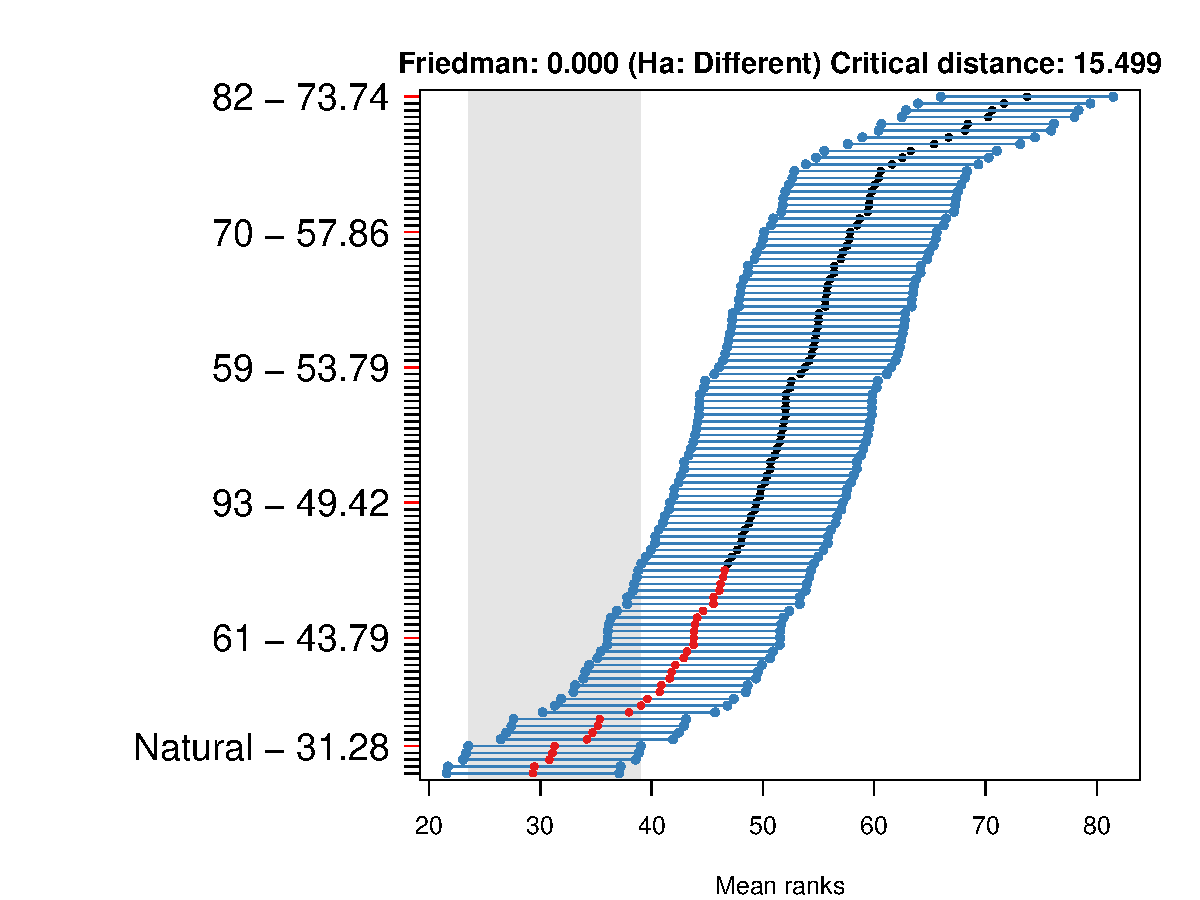
\includegraphics[width=0.45\textwidth]{../manuscript/figures/hierarchy_rmsse/tourism/P2_natural_vs_pn_h12.pdf}
	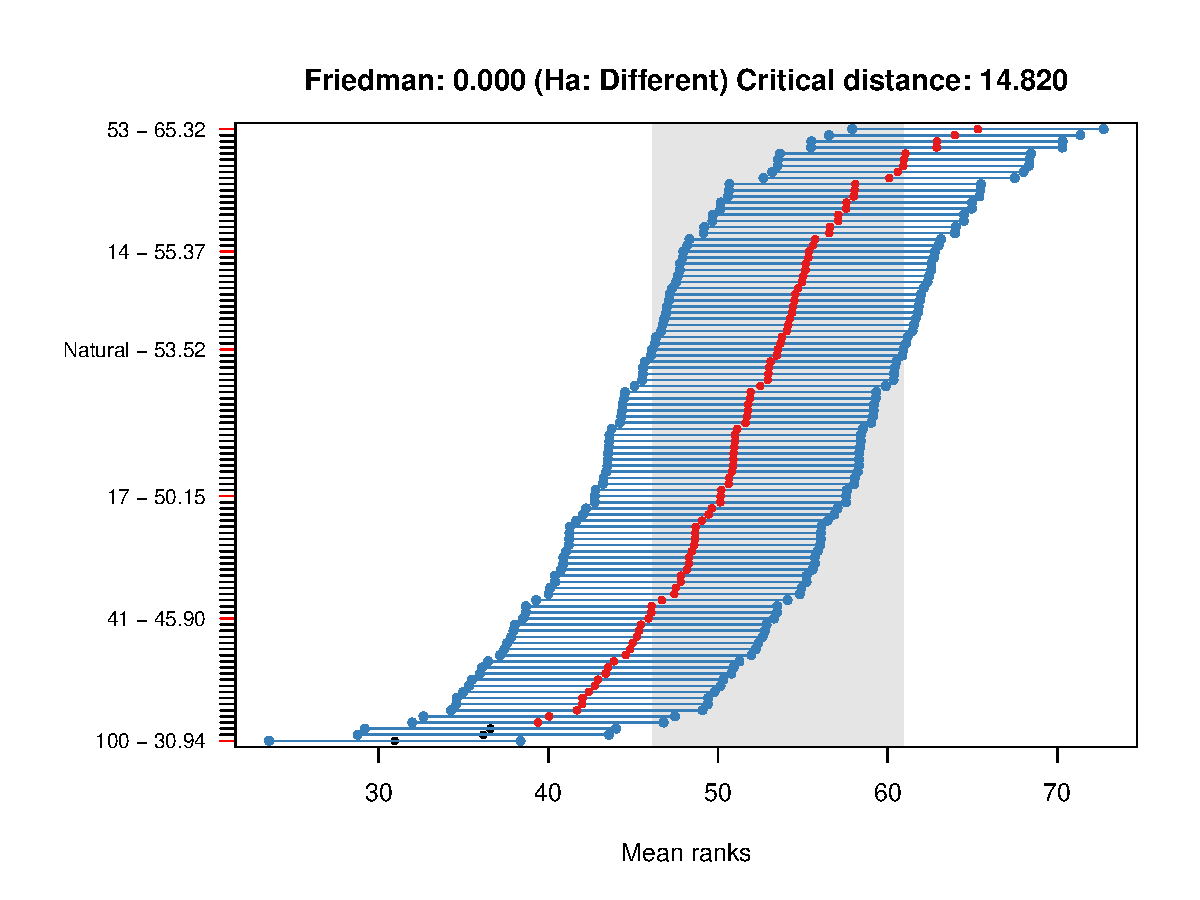
\includegraphics[width=0.45\textwidth]{../manuscript/figures/hierarchy_rmsse/mortality/P2_natural_vs_pn_h12.pdf}
	\caption{Average ranks and 95\% confidence intervals for natural hierarchy and its 100 twins, tourism dataset (left) and mortality dataset(right).}
\end{figure}
	
\end{frame}

\begin{frame}{Best cluster hierarchy vs its twins}

	We construct $100$ twin hierarchies for each of the two best cluster hierarchies and compare their performance.
	
	\begin{figure}
		\centering
		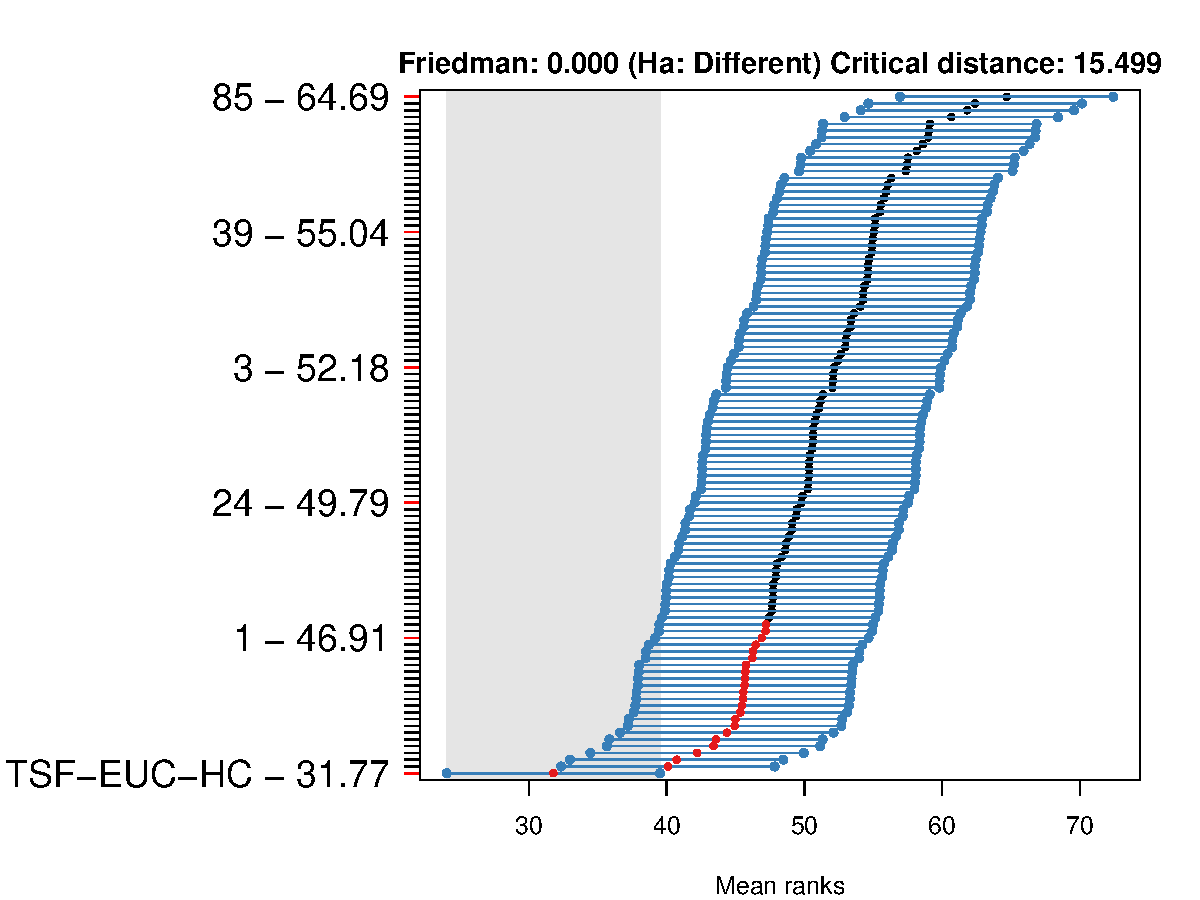
\includegraphics[width=0.45\textwidth]{../manuscript/figures/hierarchy_rmsse/tourism/P3_cluster_vs_pc_h12.pdf}
		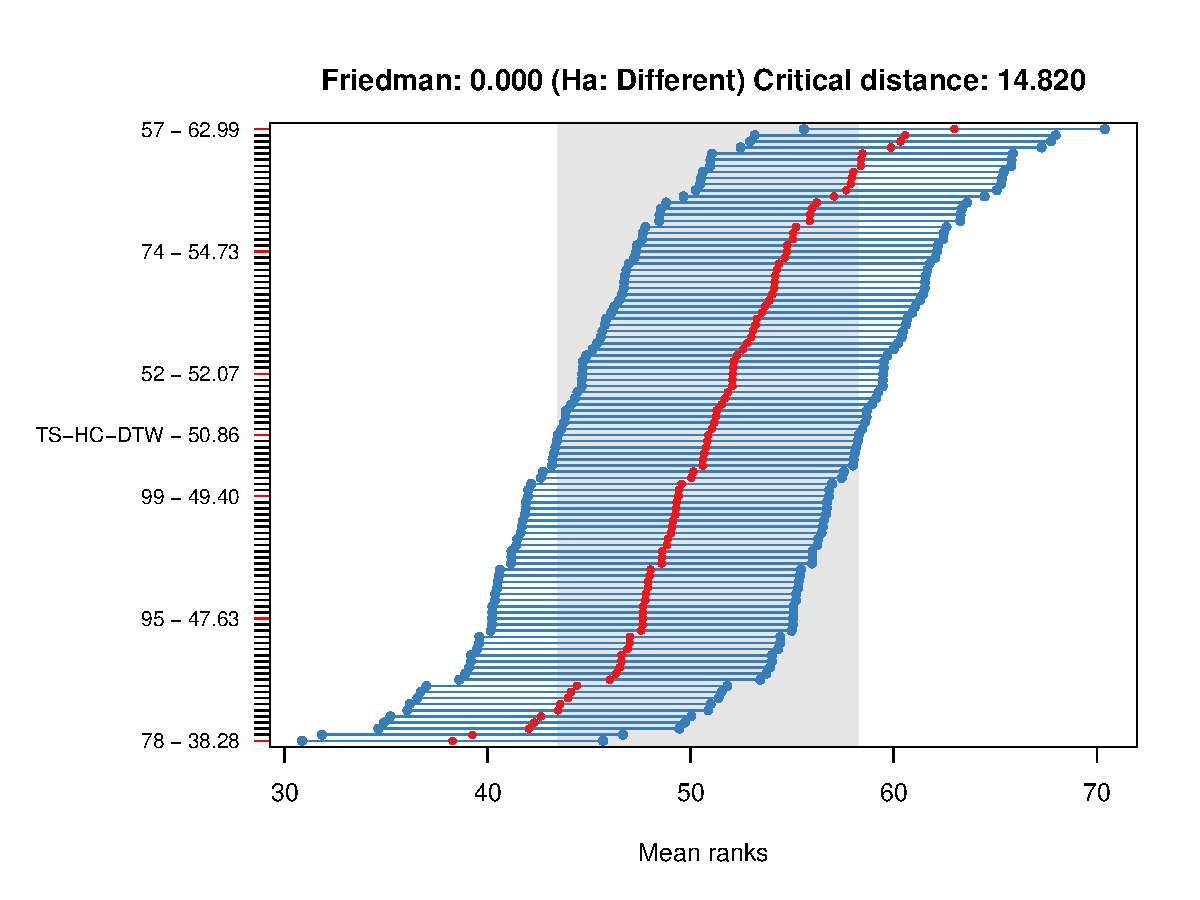
\includegraphics[width=0.45\textwidth]{../manuscript/figures/hierarchy_rmsse/mortality/P3_cluster_vs_pc_h12.pdf}
		\caption{Average ranks and 95\% confidence intervals for the best cluster hierarchy and its 100 twins, tourism dataset (left) and mortality dataset(right).}
	\end{figure}
		
	\end{frame}

\begin{frame}{Disentangling grouping and structure}
	\begin{itemize}
		\item For mortality dataset,  the performances of the natural hierarchy and the best cluster hierarchy are statistically {\color{red} indistinguishable from most of their twins}. {\color{red} ``Structure'' is the primary contributor} to the improvement in forecast accuracy over the two-level hierarchy.
		\item For tourism dataset, both natural and best cluster hierarchies are  statistically indistinguishable from around $30$ of their twins, but significantly better than the remaining $70$.
		\item For tourism dataset, {\color{red} a data-driven method} for grouping time series plays {\color{red} a more prominent role} in forecast improvement. This may be attributed to the noisier nature of bottom level tourism data, suggesting that similar weak signals are strengthened when aggregated.
		\item However, there roughly a {\color{red} 30\% chance that a random twin performs similarly}, once again highlighting that structure is the main contributor to improved forecast performance.
	\end{itemize}
\end{frame}


\begin{frame}{Forecast combination}
	\begin{itemize}
		\item Although it is possible to significantly improve forecast performance through clustering, the {\color{red} selection of the best performing combination} of time series representation, distance measure, and clustering algorithm remains an open question.
		\item We consider {\color{red} averaging forecasts across different hierarchies}, as an alternative to hierarchy selection.
	\end{itemize}
\end{frame}

\begin{frame}{Forecast combination}
	\begin{figure}
	\centering
	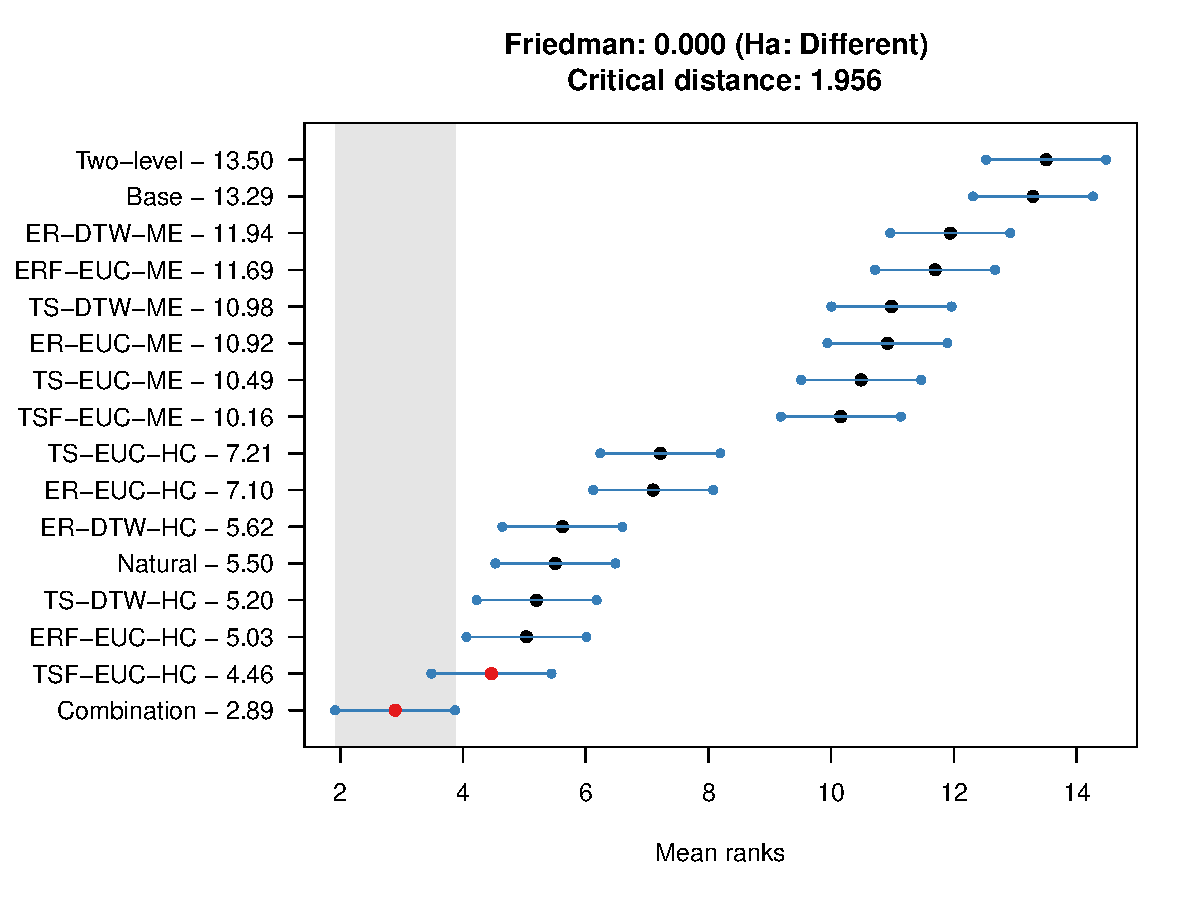
\includegraphics[width=0.45\textwidth]{../manuscript/figures/hierarchy_rmsse/tourism/P4_benchmarks_h12.pdf}
	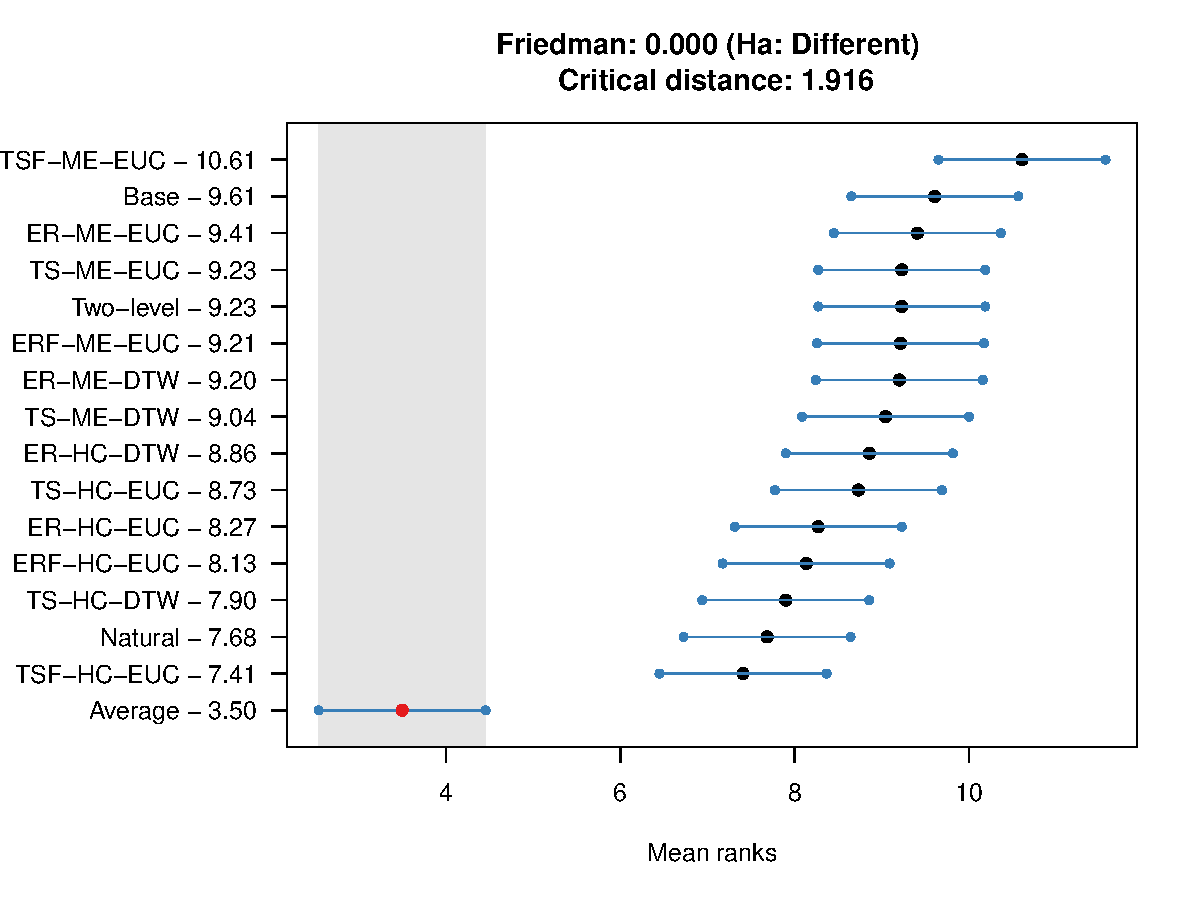
\includegraphics[width=0.45\textwidth]{../manuscript/figures/hierarchy_rmsse/mortality/P4_benchmarks_h12.pdf}
	\caption{Average ranks and 95\% confidence intervals for all approaches on tourism dataset(left) and mortality dataset(right) based on MCB test}
	\end{figure}
	\begin{itemize}
		\item On both datasets, forecast combination improves forecast performance compared to any single hierarchy. The improvement on the mortality dataset is more pronounced.
	\end{itemize}
\end{frame}

\section{Conclusions}

\begin{frame}{Conclusions}
	\begin{itemize}
		\item We consider a general framework, incorporating three distinct approaches: cluster hierarchies, permutation hierarchies, and combination hierarchies.
		\item Although adding middle-level time series via clustering or natural hierarchy improve forecast accuracy over two-level hierarchy, {\color{red}the primary contributing factor varies across datasets}. For both datasets, ``structure'' plays an important role.
		\item Our main practical recommendation is to {\color{red}use multiple clustering methods and combine forecasts across these methods using equal weights combination}. This mitigates the uncertainty of selecting the best clustering approach and is shown to significantly outperform all benchmarks across both datasets that we consider.
	\end{itemize}
\end{frame}

\begin{frame}
\frametitle{Questions and discussions}%{End of presentation}

	\vspace{-0.15in}
\begin{figure}[h!]
	\centering
	
\includegraphics[width=0.5\textwidth]{end.jpg}
	%	\caption{\normalsize{ US mortality forecasts at age 85$+$ for the period 2018--2027}}
	%	\label{fig:US_totalforecast}
\end{figure}

\Large
\begin{center}
	%\color{blue}Thank you!\\
%	\vspace{-0.1in}
	\begin{itemize}
		\centering
	%	\item[] Any questions/comments/suggestions?
		\vspace{-0.05in}
		
		\item[] \small\color{purple}Contact email: {\color{blue}   zhangbohan@buaa.edu.cn}
   
  %\\
%		\color{purple}Research Gate page:  \textit{http://www.researchgate.net/profile/Han\_Li51}
	\end{itemize}
\end{center}


\end{frame}



\begin{frame}[noframenumbering]{References}
	\bibliographystyle{agsm}
	\bibliography{../manuscript/references.bib}		
\end{frame}

\end{document}

